\documentclass[tikz]{standalone}
\usepackage{pgfplots}
\pgfplotsset{compat=1.15}
\usepackage{mathrsfs}
\usetikzlibrary{arrows,calc}
\usepackage{tkz-euclide}

\pagestyle{empty}

\definecolor{AngleClr}{rgb}{0,0.39215686274509803,0}
\definecolor{ShapeClr}{rgb}{0.6,0.2,0}

\begin{document}

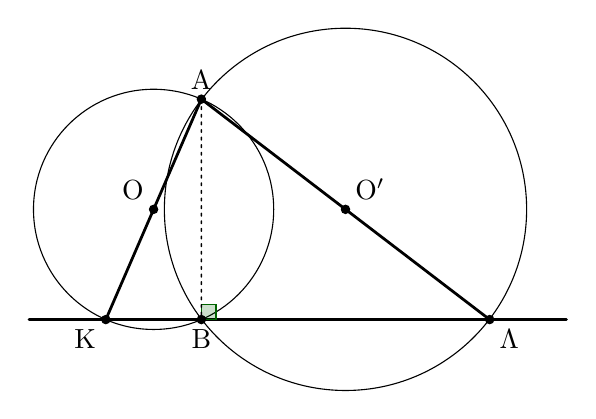
\begin{tikzpicture}[scale=.75]
\tkzSetUpLine[line width=1pt,color=black]
\tkzSetUpPoint[fill=black]

\tkzDefPoints{0/0/B,0.12/2/A,6.5/0/C}

\tkzDefTriangleCenter[circum](A,B,C) \tkzGetPoint{O}
\tkzDefPointBy[rotation=center O angle -40](A) \tkzGetPoint{P}

\tkzDefMidPoint(P,A) \tkzGetPoint{MA}
\tkzDefMidPoint(P,B) \tkzGetPoint{MB}
\tkzDefMidPoint(P,C) \tkzGetPoint{MC}

\tkzDefPointBy[projection = onto B--C](P) \tkzGetPoint{PA}
\tkzDefPointBy[projection = onto A--C](P) \tkzGetPoint{PB}
\tkzDefPointBy[projection = onto A--B](P) \tkzGetPoint{PC}

\tkzDrawSegments(P,B P,C)
\tkzDrawSegment[add=0.2 and 0.2](B,C)

% \tkzDrawCircle[color=black,line width=0.6pt](O,A)
% \tkzDrawCircles[color=AngleClr,line width=0.4pt](MA,A)
\tkzDrawCircles[color=black,line width=0.4pt](MB,B)
\tkzDrawCircles[color=black,line width=0.4pt](MC,C)

\tkzMarkRightAngles[line width=0.5pt, size=.25,color=AngleClr,fill=AngleClr,fill opacity=0.2](P,PA,C)
\tkzDrawSegments[line width=0.5pt,color=black,dashed,dash pattern=on 1pt off 1.75pt](P,PA)

\tkzDrawPoints[size=3](B,C,P,MB,MC,PA)
% \tkzLabelPoint[above left](A){$\rm A$}
\tkzLabelPoint[below left](B){$\rm K$}
\tkzLabelPoint[below right](C){$\rm \Lambda$}

\tkzLabelPoint[above left](MB){$\rm O$}
\tkzLabelPoint[above right](MC){$\rm O'$}

\tkzLabelPoint[below](PA){$\rm B$}
% \tkzLabelPoint[below left](PB){$\rm P_B$}
% \tkzLabelPoint[left](PC){$\rm P_\Gamma$}
\tkzLabelPoint[above](P){$\rm A$}

\end{tikzpicture}
\end{document}
